\documentclass{ecnreport}

\stud{M2 CORO-IMARO}
\topic{Task-based control}

\begin{document}

\inserttitle{Task-based control lab}

\insertsubtitle{Robot arm control}

\section{Content of this lab}

The goal of this lab is to control one arm of the Baxter robot, first in simulation then on the real robot.

The robot is simulated with Gazebo\footnote{https://gazebosim.org}.
In the simulation is placed a green sphere. The goal is to move the arm so that the sphere is centered and at a given distance from the camera.
The robot control will be performed in C++ and will rely on:

\begin{itemize}
 \item The ROS framework to handle communication between the simulator and the control program (actually hidden inside the robot class).
 \item The ViSP library\footnote{Visual Servoing Platform, http://visp.inria.fr} to manipulate vectors and matrices and to perform linear algebra.
\end{itemize}
The actual classes that are used are detailed in Appendix \ref{sec:classes}.\\

\subsection{Environment setup}

ROS environment should already be set up in the computers. You can setup Qt Creator or VS with the \okt{ros_management_tools}\footnote{https://github.com/oKermorgant/ros\_management\_tools}:

\begin{bashcodelarge}
 # go to the tbc_baxter_vs folder
 colbuild -t # compiles this package
 ideconf # build the configuration file for Qt Creator and VS code
\end{bashcodelarge}

\subsection{Structure of the \okt{tbc_baxter_vs} package}

The only file to be modified is \okt{main.cpp}, which is the main file for the C++ program. \\
The simulation can be launched with: \okt{roslaunch tbc_baxter_vs sim.launch}.

We can see that the simulator sends the joint states and the camera image to the control node. In return, the control node sends the joint setpoints
to the simulator.\\

The simulation can be run with a moving ball with: \okt{roslaunch tbc_baxter_vs sim.launch manual:=false}.

\subsection{The Baxter robot (arm)}

The considered robot is one arm of Baxter. A camera is placed at inside the end-effector of the robot.
 The robot is controlled through joint velocity $\dot \q$.
 In the initial state of the control node, the error and interaction matrix are not computed, inducing a null joint velocity setpoint.
 
\section{Expected work}

\subsection{Basic visual servoing}

The first goal is to actually compute a classical visual servoing. The features are defined as $\s = (x, y, a)$ where $(x,y)$ is the position of the center of gravity of the sphere and $a$ is its area in the image.

The current features are accessed through \okt{arm.x(), arm.y(), arm.area()} while the desired ones are set to 0 for $(x,y)$ and accessed through \okt{arm.area_d()} for the area.
The error vector \okt{e} has to be defined from the current and desired features.

Similarly, the interaction matrix of $\s$ should be defined in \okt{L}. The feature Jacobian, that expresses the time-variation of $\s$ with regards to $\dot \q$ should then be computed
from \okt{L} and \okt{arm.cameraJacobian()}.

The desired joint velocities can then be computed with $\dot \q = -\lambda\J^+\e$. Of course this control law does not take into account the joint limits. \\The gain $\lambda$ should be equal to \okt{arm.lambda()}, in order to be tuned online.

\subsection{Feedforward term}

When observing a moving object, the proportional control will always lag behind the object. One way is to increase the gain to have a more reactive control but might get instable. Another way is to try and identify the motion of the object in the image and use a feedforward to compensate. You can implement this part in the \okt{if(use_feedforward)} block.

\subsection{Avoiding useless rotations}

The sphere-based features allow any rotation around the Z-axis of the camera as it does not change the object in the image.
In order to stabilize the system we can add a constraint that is having the X-axis of the camera orthogonal to the Z-axis of the base frame.

The rotation matrix $\Pass{b}{\R}{c}$ can be obtained with:
\begin{cppcode}
 const auto bRc = arm.cameraPose().getRotationMatrix();
\end{cppcode}
Knowing that $\Pass{b}{\dot\R}{c} = \Pass{b}{\R}{c}\skew{\boldsymbol\omega_c}$, express the interaction matrix of this new feature and add it to the control.

\subsection{Visual servoing with joint limits}

We will use the augmented Jacobian framework\footnote{O. Kermorgant, F. Chaumette. Dealing with constraints in sensor-based robot control. In IEEE Trans. on Robotics, Feb 2014}.
In this framework, the constraints are modeled as additional sensor features. The desired value simply corresponds to the avoidance direction, and can usually be defined by using the center of the valid interval: $\q^* = \frac{1}{2}(\q^+ + \q^-)$.

A safe interval $(\q^{s-}, \q^{s+})$ has to be defined with a margin $\rho\in]0.,0.5[$ with:
\begin{equation*}
\left\{\begin{array}{ll}
	\q^{s+} = & \q^{+} - \rho(\q^+ - \q^-) \\
	\q^{s-} = & \q^{-} + \rho(\q^+ - \q^-)
\end{array}\right.
\end{equation*}$\rho$ can be set to e.g. 5 to 10\%.\\

The classical weighting function is depicted in \Fig{weight}. It is available in the code, as the \okt{h_weight} function:
\begin{equation*}
 h(s, s_{\text{act}}, s_{\max}) = \left\{\begin{array}{ll}
       h(-s, -s_{\text{act}}, -s_{\max}) & \text{if } s_{\text{act}} \ge s_{\max} \\
       0 & \text{if } s < s_{\text{act}} \\
    \displaystyle  \frac{s-s_{\text{act}}}{s_{\max}-s} & \text{otherwise}
                                         \end{array}\right.
\end{equation*}

\begin{figure}[h]\centering
	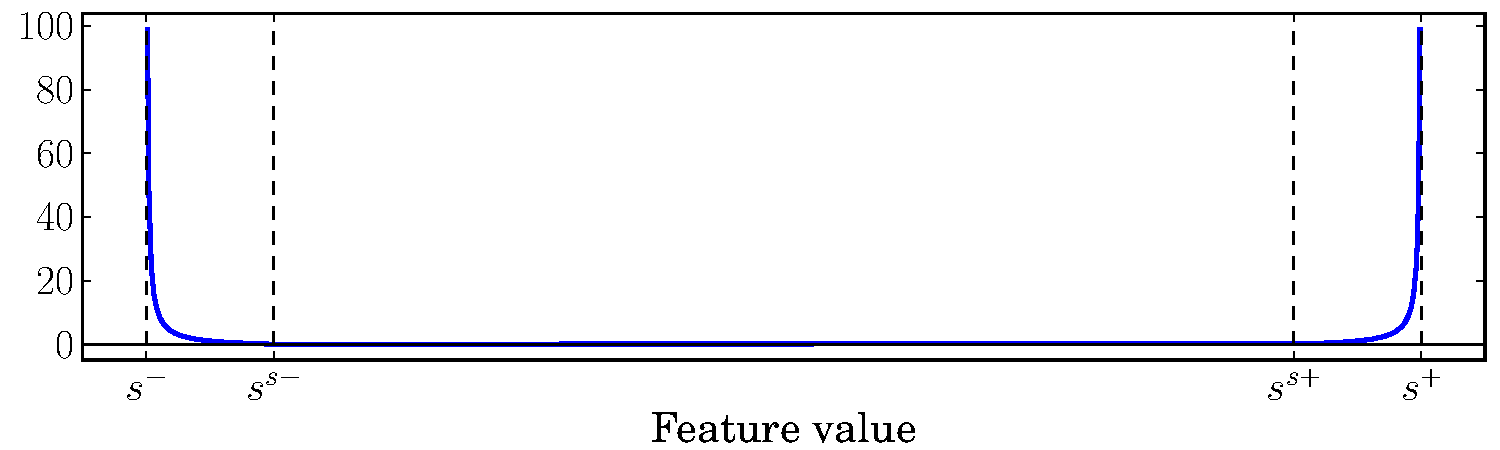
\includegraphics[width=.7\linewidth]{constraint_0inf}
	\caption{Typical weighting function from $(s^-, s^{s-}, s^{s+}, s^+)$}
	\label{weight}		
\end{figure}

The control then yields: 
\begin{center}
	$\dot \q = \arg\min \norm{\H\tilde\J\dot \q + \lambda\H\tilde\e}^2$ \\
 where: $\H = \left[\begin{array}{cc}\I_4 & 0 \\ 0 & \diag{h_i}\end{array}\right]$,
 $\tilde\J = \left[\begin{array}{c}\J \\ \I_n \end{array}\right]$ and
  $\tilde\e = \left[\begin{array}{c}\e \\ \q - \q^* \end{array}\right]$
\end{center}
The solution to the minimization can be explicitly written as $\dot \q = -\lambda(\H\tilde\J)^+\H\tilde\e$.\\

\subsection{Visual servoing and joint control with joint limits }

If we use the above formulation then the robot avoids its joint limits but the control law may be discontinuous. Indeed, $(\H\tilde\J)$ is a $11\times 7$ matrix whose rank may vary from 4 (all joints in their safe zone) to 7 (at least 3 joints close to their limits). A solution is to set arbitrary values for 3 joints. \\

A good choice is to use the default value (output of \okt{arm.init()}) as desired value for joints $3\hdots7$ and keep their weight equal to 1.
The joints $1\hdots 4$ will be used for the visual servoing while avoiding their limits.

\subsection{Use on the real robot}

If the simulation is working fine, you can control the real robot simply by connecting to the rosmaster of the robot. This is done in a terminal with:
\begin{bashcodelarge}
 ros_baxter
\end{bashcodelarge}A \okt{[baxter]} text should appear in the prompt and for all new terminals afterwards.\\
Then just the Baxter bridge from the same terminal:
\begin{bashcodelarge}
 ros2 run baxter_bridge bridge
\end{bashcodelarge}This node will transfert ROS 2 topics to good old ROS 1 topics that Baxter still uses.

You can then run your node from another terminal of the IDE.
\begin{bashcodelarge}
 ros2 run tbc_baxter_vs baxter_vs
\end{bashcodelarge}

You can also indicate whether you want to control the left or right arm. The visual detector is designed to detect green objects on the right camera and red objects on the left one. An additional image processing window will open in order to tune the Hue and Saturation thresholds, that may depend on the light conditions of the room.\\

If you want to go back to a local simulation, you can run the following line:
\begin{bashcodelarge}
 ros_reset
\end{bashcodelarge} It will be valid for all new terminals afterwards.

\appendix

\section{Main classes and tools}\label{sec:classes}

\subsection{ViSP classes}

This library includes many tools for linear algebra, especially for 3D transformations. 
The documentation is found here: \url{http://visp-doc.inria.fr/doxygen/visp-daily/classes.html}.\\
The main classes from ViSP (at least in this lab) are:
\begin{itemize}
\item \okt{vpFeaturePoint} (variable \okt{p}) represents a Cartesian 2D point as feature. It can be updated with \okt{p.set_xyZ(x,y, 1);}. The main interest is that the corresponding $2\times 6$ interaction matrix can be retrieved by \okt{p.interaction();}
\item \okt{vpMatrix} represents a classical matrix, can then be transposed, inversed (or pseudo-inversed), multiplied with a vector, etc.
\item \okt{vpColVector} is a column vector with classical mathematical properties.
\end{itemize}
These class can be declared and used as follows:
\begin{cppcode}
       vpMatrix M(2,6); 	// matrix of dim. 2x6
       M[0][0] = M[1][1] = 1;	// element-wise assignment
       vpColVector v(6);	// column vector of dim. 6
       v[0] = 1;		// element-wise assignment
       M*v;			// matrix-vector multiplication
\end{cppcode}

Smaller matrices and vectors can be inserted or extracted:

\begin{cppcode}
       vpMatrix M(2,6);
       auto Msub = M.extract(0,0,1,2);     // extracts the 1st row and 2 first columns, Msub is 1x2
       M.insert(Msub, 1,2);                // inserts Msub into M, starting at row 1, col 2

       vpColVector v(6);	// column vector of dim. 6
       auto Vsub = v.extract(1,3); // extracts elements at indices (1,2,3)
       v.insert(0,Vsub);                  // inserts Vsub into v at row 0
\end{cppcode}



%
%\subsection{The Baxter class}
%\label{baxter}
%The Baxter class hides all the ROS communication aspects in order to have a higher-level access. As this is not a lab on robot modeling, all Jacobians are already 
%available - even if it could be a nice exercice to compute the camera Jacobian. 
%
%The main methods of the \okt{Baxter} class can be seen in the \okt{baxter_arm.h} file:
%\begin{itemize}
% \item Getters for robot model or measurements:
% \begin{itemize}
%  \item \okt{double robot.radius()}, \okt{robot.base()}, \okt{robot.wmax()} : kinematic model.
%  \item \okt{void robot.getImagePoint(vpColVector \&)}: get the measured center of gravity of the sphere in the image, in normalized coordinates.
%  \item \okt{vpColVector robot.getCamLimits()}: get the upper bounds for $(x,y)$. Lower bounds are the opposite.
%  \item \okt{vpMatrix robot.getCamJacobian()}: get the Jacobian between the camera velocity screw in its own frame and the robot command $\dot \q$. This Jacobian is to be multiplied
%  by the interaction matrix of a point to get the actual Jacobian of the image coordinates with regards to the robot command.
% \end{itemize}
%\item \okt{robot.setVelocity(vpColVector)}: send a $\dot \q$ velocity. Wheel velocity limits will be applied before actually sending it to the simulator.
%\end{itemize}

% 
% \begin{itemize}
%  \item \okt{setVelocity(vpColVector)}: sends a $(v, \omega, \dot q_p, \dot q_t)$ velocity to the robot, wheels velocity limits will be ensured
%  \item \okt{getImagePoint(vpColVector \&)}: gives the current position (normalized coordinates) of the sphere in the image
% \end{itemize}






\end{document}
